\section{Roadmap timeline and dependency graph}\label{sec:E-roadmap-timeline}

\texttt{flux-roadmap-public.\allowbreak{}md} is InFlux Technologies' public roadmap document and is treated
throughout this appendix as the single source of truth for committed items; a separate,
hand-authored file, \texttt{timeline.html}, carries roughly two dozen additional items with no
corresponding prose and is reported only as a weaker, non-committed signal in \S\ref{sec:E4}.
The document states its own attribution as ``Published July 2026, updated August 2026, by InFlux
Technologies'' \srcdoc{flux-roadmap/public/flux-roadmap-public.md:223}. The \emph{assessment}
column added to every table below is this paper's own evidence-bound reading of a roadmap item's
stated status — tagged for provenance, hedged wherever the underlying evidence is thin, and never
treated as grounds to mark an item \shipped on the roadmap's authority alone.

Pillar codes (P1--P9) are reproduced verbatim from the roadmap's own item table, which does not
carry a legend. The extraction corpus does use them consistently, with a parenthetical gloss on
almost every occurrence, so the legend below is reconstructed from that usage rather than invented or
left undefined. It is marked \srcinferred{} because it is a reconstruction: no single artefact states
it.

\begin{table}[H]
\centering\footnotesize
\caption{Pillar codes as used throughout the extraction corpus. Reconstructed from consistent
parenthetical glosses across \texttt{evidence/*.md}; no source states the mapping directly.
\srcinferred{} \srcdoc{evidence/*.md, pillar annotations}.}
\label{tab:pillar-legend}
\begin{tabular}{@{}ll@{}}
\toprule
Code & Scope as used in the corpus \\
\midrule
P1 & Consensus and the chain --- \fluxd, tiering, collateral, pruning \\
P2 & Monetary policy --- emission, \PNR, parallel-asset consolidation \\
P3 & Flux Cloud substrate --- \FluxOS, app lifecycle, billing, Deploy-from-Git \\
P4 & Network and addressing --- FDM, PDNS, mesh resolution, port and IP policy \\
P5 & Attested execution --- \ArcaneOS, \SAS, measured boot \\
P6 & Accelerated compute and AI tenancy --- GPU, inference, the agent-facing interface \\
P7 & Governance and moderation \\
P8 & Value transfer and privacy --- bridge, shielded notes, wallet and key stack \\
P9 & Vertical integration --- the coupling of chain, \FluxOS{} and \ArcaneOS \\
\bottomrule
\end{tabular}
\end{table}

%% =====================================================================
\subsection{Committed items}\label{sec:E1}

Each table reproduces, verbatim where quoted, the Name / Pillar / Maturity / Dependency columns of
the roadmap's own item table, one \texttt{longtable} per stated quarter, in the roadmap's own
order. The \S and Assessment columns are this paper's addition. ``\S\ref{sec:feasibility}'' below
refers to this paper's feasibility section and its mechanism table (\Cref{tab:feasibility});
mechanism numbers and classes (Extension / Engineering / Research) are cited from that table where
a roadmap item matches one of its rows.

\begingroup
\footnotesize
\setlength{\tabcolsep}{4pt}
\begin{longtable}{p{0.15\linewidth}p{0.05\linewidth}p{0.14\linewidth}p{0.19\linewidth}p{0.05\linewidth}p{0.24\linewidth}}
\caption{Q3 2026 (``shipping now''), committed items per \texttt{flux-roadmap-public.\allowbreak{}md}.}\label{tab:e1-q3}\\
\hline
\textbf{Item} & \textbf{Pillar} & \textbf{Roadmap maturity} & \textbf{Dependency} & \textbf{\S} & \textbf{Assessment} \\
\hline
\endfirsthead
\multicolumn{6}{l}{\textit{Table \thetable\ continued}}\\
\hline
\textbf{Item} & \textbf{Pillar} & \textbf{Roadmap maturity} & \textbf{Dependency} & \textbf{\S} & \textbf{Assessment} \\
\hline
\endhead
\hline
\endfoot
\hline
\endlastfoot
CumulusVPN (network) & P8, P4 & SHIPPED-per-roadmap (``The network is live'') \srcdoc{flux-roadmap/public/flux-roadmap-public.md:13,15-18} & Apple/Google app-store review for client apps & \S16 & Operational status is consistent with a shipped, live payment-gated gateway fleet: CumulusVPN's payment-derived entitlement runs end to end in code (\S16, C19), though a linkability caveat noted there is not addressed by this roadmap text (\S21). \\
CumulusVPN apps (iOS/Android/macOS) & P8 & IN-PROGRESS-per-roadmap (``in store review'') \srcdoc{flux-roadmap/public/flux-roadmap-public.md:16,18} & Apple's and Google's review queues & Outside this paper's scope (client app-store release process) & \decided{app-store reviews are \textbf{done} \srcintent{08-answers-round-2.md, round 23}} \\
AmneziaWG obfuscation / WireGuard-over-TLS / multi-hop / stealth transport (port 443) & P4, P8 & SHIPPED-per-roadmap (``Already in the gateways'') \srcdoc{flux-roadmap/public/flux-roadmap-public.md:20} & none stated & \S16 (indirect) & The CumulusVPN gateway fleet is independently evidenced as live and payment-gated (\S16, C19), consistent with an operational gateway, but the AmneziaWG/WireGuard-over-TLS transport claim itself has no direct counterpart in this paper's corpus. \\
SSP v2 (wallet redesign) & P8 & IN-PROGRESS-per-roadmap (described as a redesign, not marked live) \srcdoc{flux-roadmap/public/flux-roadmap-public.md:22-23} & none stated & \S17 (indirect) & This paper's SSP evidence covers only the existing, pre-redesign signing architecture, where the SSP and ZelCore paths sign locally on-device (\S17, C20); it says nothing about a \emph{v2} redesign specifically. \\
Flux Console (enterprise) & P3, P7 & SHIPPED-per-roadmap (``Live with our largest clients'') \srcdoc{flux-roadmap/public/flux-roadmap-public.md:25-28} & none stated & Outside this paper's scope (enterprise console product) & \decided{Flux Console is \textbf{built} \srcintent{08-answers-round-2.md, round 23}; no artefact in this paper's corpus covers it, so nothing here describes its behaviour} \\
Tokenised equities in Zelcore (bStocks) & P8 & IN-PROGRESS-per-roadmap \srcdoc{flux-roadmap/public/flux-roadmap-public.md:30-31} & ``ahead of the September deadline'' (external regulatory deadline) & Outside this paper's scope (tokenised-equities product) & \decided{\textbf{not built} as of 2026-09-06 \srcintent{08-answers-round-2.md, round 23}; the absence of corpus evidence reflects that, not a gap in this survey} \\
RPC, archive and indexing services & P3, P1 & PLANNED (``first capacity-selling product'') \srcdoc{flux-roadmap/public/flux-roadmap-public.md:33-34} & Stated to pair with main-chain pruning (H1 2027) & \S\ref{sec:feasibility} (\#6) & The dependency, main-chain pruning, is independently classed Extension: \texttt{-prune} is already wired and the FluxNode registry sits in a separate store (\S\ref{sec:feasibility}, mechanism 6); archive-node economics remain the open sub-problem. \\
Supply transparency / live supply tracker & P2 & IN-PROGRESS (repository built; public deployment not verified) \srccode{flux-supply-tracker/\allowbreak{}README.md}{1--3}\srcdoc{flux-roadmap/public/flux-roadmap-public.md:36-37} & none stated & \S5, \S6 & The roadmap's own reconciliation places issued supply within 0.0005\% of the emission model \srcroadmap{flux-roadmap-public.md:185}, and \S5 finds the paper's computed supply consistent with it, but two existing tracker implementations exclude team-reserve wallets using disagreeing lists (C18) — directly relevant to what a ``live'' tracker would need to reconcile. \\
\end{longtable}
\endgroup

\begingroup
\footnotesize
\setlength{\tabcolsep}{4pt}
\begin{longtable}{p{0.15\linewidth}p{0.05\linewidth}p{0.14\linewidth}p{0.19\linewidth}p{0.05\linewidth}p{0.24\linewidth}}
\caption{Q4 2026 (``the platform becomes one product''), committed items per \texttt{flux-roadmap-public.\allowbreak{}md}.}\label{tab:e1-q4}\\
\hline
\textbf{Item} & \textbf{Pillar} & \textbf{Roadmap maturity} & \textbf{Dependency} & \textbf{\S} & \textbf{Assessment} \\
\hline
\endfirsthead
\multicolumn{6}{l}{\textit{Table \thetable\ continued}}\\
\hline
\textbf{Item} & \textbf{Pillar} & \textbf{Roadmap maturity} & \textbf{Dependency} & \textbf{\S} & \textbf{Assessment} \\
\hline
\endhead
\hline
\endfoot
\hline
\endlastfoot
FluxCloud + FluxEdge merged into one product & P3 & PLANNED \srcdoc{flux-roadmap/public/flux-roadmap-public.md:41,43-44} & none stated & \S\ref{sec:feasibility} (\#21) & Classed Engineering: ``two runtimes and two products today''; convergence is organisational as much as technical (\S\ref{sec:feasibility}, mechanism 21). \\
Rebuilt interface (signup$\to$deploy$\to$payment$\to$domain) & P3 & PLANNED \srcdoc{flux-roadmap/public/flux-roadmap-public.md:46-47} & Depends on the FluxCloud+FluxEdge merge & \S\ref{sec:one-platform} (indirect) & \decided{\textbf{not built} as of 2026-09-06 \srcintent{08-answers-round-2.md, round 23}; the absence of corpus evidence reflects that, not a gap in this survey} \\
One balance, everywhere (top-ups, auto-renew, low-balance warnings, grace period) & P3, P2 & PLANNED \srcdoc{flux-roadmap/public/flux-roadmap-public.md:49-50} & none stated & \S\ref{sec:feasibility} (\#11) & Classed Engineering (\S\ref{sec:feasibility}, mechanism 11): an auto-renewal precedent already exists (\texttt{appsmonitor}, Foundation-held keys), but a self-custodied balance and its grace/suspension/eviction state machine do not. \\
FluxOS v9 application specifications & P3 & IN-PROGRESS-per-roadmap (``well underway, with the routing layer already rewritten against it and a full regression suite in place'') \srcdoc{flux-roadmap/public/flux-roadmap-public.md:52-53,66} & Published as an RFC before rollout; ``tested like consensus code'' — implies a network-wide agreement gate & \S10, \S\ref{sec:feasibility} (\#5) & See \S\ref{sec:E2} (C4): substantially supported (932 changed files, 7,763 test cases per push), but the work lives on a contributor fork rather than the organisation repository, its enforcement height was settled only later at $\hstar = \num{3050000}$ (\S\ref{sec:appspec-v9}), and three of the five new required fields have no consumer code. \\
v9: cleaner deployment model (named component map; \texttt{image}, \texttt{cpu}, \texttt{memory}, \texttt{rootFsGb}; named ports) & P3 & PLANNED (sub-item of v9) \srcdoc{flux-roadmap/public/flux-roadmap-public.md:57} & Part of v9 & \S10 & Sub-item of v9; see \S\ref{sec:E2} for the parent claim's status. \\
v9: real load balancing (per-route HTTP/TCP config, HTTPS redirect, custom domains, managed certs, health checks, timeouts, sticky sessions, connection limits, retries, backend TLS w/ per-app CAs, connection draining) & P3, P4 & PLANNED \srcdoc{flux-roadmap/public/flux-roadmap-public.md:58} & Part of v9 & \S10 & The fork wires connection-draining and per-app-CA backend TLS under the \texttt{loadBalancing} block, but FluxOS itself contains no HAProxy config-generation engine — that stays in FDM (C4). \\
v9: persistent storage (sized volumes, explicit mount mapping) & P3 & PLANNED \srcdoc{flux-roadmap/public/flux-roadmap-public.md:59} & Part of v9 & \S10 & Sub-item of v9; no independent evidence beyond the parent claim in \S\ref{sec:E2}. \\
v9: replicas and placement (active-standby, active-active, sync-before-start ordering) & P3 & PLANNED \srcdoc{flux-roadmap/public/flux-roadmap-public.md:60} & Part of v9 & \S10 & The mastership/active-standby quorum plane (\texttt{quorum\allowbreak{}Grant\allowbreak{}Activation\allowbreak{}Height}) is read by production code but set only in test fixtures and absent from shipped config (C4). \\
v9: cleaner encryption envelope for private specs & P3, P5 & PLANNED \srcdoc{flux-roadmap/public/flux-roadmap-public.md:61} & Part of v9 & \S10, \S20 & The draft schema removes v8's \texttt{enterprise} field with no replacement and defines no signature field, with canonicalization only recommended rather than enforced (C4a) — this promise is currently unmet in the draft this paper reviewed. \\
v9: Duration as first-class field & P3, P2 & PLANNED \srcdoc{flux-roadmap/public/flux-roadmap-public.md:62} & ``Foundation the subscription and auto-renew work builds on'' & \S10 & Stated foundation for the One-balance/auto-renew item above; consumer code for this field was not found in this paper's corpus (C4). \\
v9: payment memo field & P2, P3 & PLANNED \srcdoc{flux-roadmap/public/flux-roadmap-public.md:64} & ``The basis for paying operators under PNR v2'' & \S7, \S10 & Zero consumer code anywhere in FluxOS for this field (C4); it is the field PNR v2 is stated to depend on — see \S\ref{sec:E2}. \\
v9: referral attribution field & P3 & PLANNED \srcdoc{flux-roadmap/public/flux-roadmap-public.md:64,128} & ``Preview environments and referrals'' (H1 2027) rides this field & \S10 & Zero consumer code anywhere in FluxOS for this field (C4). \\
v9: machine-type flag for VPS tier & P3 & PLANNED \srcdoc{flux-roadmap/public/flux-roadmap-public.md:64} & VPS tier (H1 2027) depends on this flag & \S10 & Zero consumer code anywhere in FluxOS for this field (C4). \\
Deploy from Git, finished & P3 & IN-PROGRESS-per-roadmap (``remaining work is hardening the build path'') \srcdoc{flux-roadmap/public/flux-roadmap-public.md:68-69} & none stated & \S17, \S19 & The \texttt{deploy-\allowbreak{}with-\allowbreak{}git-\allowbreak{}frontend} repository underlying this product family already ships MCP-based deployment tooling and signs via a remote, custodial path on one of two available routes (\S17, \S19, C20); it also generates specifications referencing a non-digest-pinned \texttt{orbit:latest} image (C20). \\
Managed databases (Postgres, MongoDB, backup/restore) & P3 & PLANNED \srcdoc{flux-roadmap/public/flux-roadmap-public.md:71-72} & none stated & \S\ref{sec:managed-services} & Two database operators a tenant deploys with its own application, \texttt{Flux-Shared-DB} and \texttt{flux-\allowbreak{}pg-\allowbreak{}cluster}, already ship (\S\ref{subsec:managed-db-comparison}); neither is the managed-database \emph{product} this item describes, which remains planned. \\
Agent-native cloud --- MCP server & P6, P3 & PLANNED \srcdoc{flux-roadmap/public/flux-roadmap-public.md:74-77} & ``Official SDKs, a real command-line interface, a Terraform provider and a GitHub Action follow from the same API'' & \S17, \S19, \S\ref{sec:feasibility} (\#14) & This paper's evidence records an MCP server already shipped in \texttt{deploy-\allowbreak{}with-\allowbreak{}git-\allowbreak{}frontend}, exposing \texttt{deploy\_app}, \texttt{update\_app} and \texttt{renew\_app} tools with remote custodial signing on one path (\S17, \S19, C20) — earlier than this item's stated placement. \\
Agent-native cloud --- Payment is the account & P6, P2 & PLANNED \srcdoc{flux-roadmap/public/flux-roadmap-public.md:78} & none stated & \S16, \S\ref{sec:feasibility} (\#13) & A form of this already ships in CumulusVPN, where a payment memo is itself the credential (\S16, C19); bounding an agent's \emph{spending}, as opposed to its actions, remains Research-classed on the L1 (\S\ref{sec:feasibility}, mechanism 13). \\
Agent-native cloud --- per-second GPU without an account & P6 & PLANNED \srcdoc{flux-roadmap/public/flux-roadmap-public.md:79} & ``With FluxEdge folded into the platform'' — depends on the FluxCloud+FluxEdge merge & \S15, \S\ref{sec:feasibility} (\#20) & GPU isolation today is whole-device only via Kubernetes passthrough, with no MIG/vGPU/time-slicing, and the requested resource is silently stripped rather than queued or rejected on contention (\S15, C23) — both bear on a per-second, no-account offering. \\
Private deployments (VPONs) & P4, P8 & PLANNED \srcdoc{flux-roadmap/public/flux-roadmap-public.md:83-84} & Described as ``the complement to private payments and chain privacy'' \srcinferred: sequenced alongside, not strictly gated & \S\ref{sec:networking} & \decided{\textbf{not built} as of 2026-09-06 \srcintent{08-answers-round-2.md, round 23}; the absence of corpus evidence reflects that, not a gap in this survey} \\
Operator protection --- application oracle & P7 & PLANNED \srcdoc{flux-roadmap/public/flux-roadmap-public.md:86,89} & none stated & \S\ref{sec:governance} & Operator-side defence; distinct from the network-side moderation quorum this paper models, which is absent from the public roadmap (\S23, C5). \\
Operator protection --- resource guardrails & P7, P1 & PLANNED \srcdoc{flux-roadmap/public/flux-roadmap-public.md:90} & none stated & \S\ref{sec:governance} & \decided{\textbf{not built} as of 2026-09-06 \srcintent{08-answers-round-2.md, round 23}; the absence of corpus evidence reflects that, not a gap in this survey} \\
Operator protection --- optional standard egress profile & P7, P4 & PLANNED \srcdoc{flux-roadmap/public/flux-roadmap-public.md:91} & none stated & \S\ref{sec:governance} & \decided{\textbf{not built} as of 2026-09-06 \srcintent{08-answers-round-2.md, round 23}; the absence of corpus evidence reflects that, not a gap in this survey} \\
Operator protection --- evidence pack & P7 & PLANNED \srcdoc{flux-roadmap/public/flux-roadmap-public.md:92} & none stated & \S\ref{sec:governance} & \decided{\textbf{not built} as of 2026-09-06 \srcintent{08-answers-round-2.md, round 23}; the absence of corpus evidence reflects that, not a gap in this survey} \\
Bridge redesign, audited (mint-and-burn) & P8, P2 & PLANNED, explicitly gated \srcdoc{flux-roadmap/public/flux-roadmap-public.md:96-97} & ``Independent audit before deploy'' — hard gate stated & \S6, \S8, \S22, \S\ref{sec:feasibility} (\#3) & This paper's bridge-design work finds the L1 header format itself forecloses the most trust-minimizing (light-client) bridge architecture until a node-set commitment is added (\S8, \S22, C26) — a constraint an audited mint-and-burn design does not by itself resolve. \\
Attestation-linked proof-of-reserve on bridge contracts & P5, P8, P2 & PLANNED \srcdoc{flux-roadmap/public/flux-roadmap-public.md:99} & Built on the bridge redesign above & \S14, \S\ref{sec:feasibility} (\#4) & Framed as the bonded attestation network's first customer (H1 2027 item below); see \S\ref{sec:E2} for the attestation dependency. \\
Privacy groundwork (technical/legal/exchange, plan published) & P8 & PLANNED \srcdoc{flux-roadmap/public/flux-roadmap-public.md:101-102,158} & Precedes H2 2027 chain privacy implementation, ``on the schedule set by the Q4 2026 plan'' & \S20, \S\ref{sec:migration} & See \S\ref{sec:E2} (C28): the shielded pool has been closed to new entrants since height 835,554, and the settled decision is to retire both pools rather than reopen them (\S\ref{sec:shielded-retirement}), so the consensus change this groundwork must schedule is a sunset, not a reopening. \\
CumulusVPN payments (in-app purchase, card) and gateway v2 & P8, P2 & PLANNED \srcdoc{flux-roadmap/public/flux-roadmap-public.md:104-105} & none stated & \S16, \S\ref{sec:feasibility} (\#10) & Direct per-deployment payment is independently classed Extension and already shipped twice, including via CumulusVPN's memo-derived entitlement (\S16, \S\ref{sec:feasibility} mechanism 10, C19); the in-app-purchase and gateway-v2 specifics are not separately evidenced. \\
\end{longtable}
\endgroup

\begingroup
\footnotesize
\setlength{\tabcolsep}{4pt}
\begin{longtable}{p{0.15\linewidth}p{0.05\linewidth}p{0.14\linewidth}p{0.19\linewidth}p{0.05\linewidth}p{0.24\linewidth}}
\caption{H1 2027 (``the chain changes''), committed items per \texttt{flux-roadmap-public.\allowbreak{}md}.}\label{tab:e1-h1}\\
\hline
\textbf{Item} & \textbf{Pillar} & \textbf{Roadmap maturity} & \textbf{Dependency} & \textbf{\S} & \textbf{Assessment} \\
\hline
\endfirsthead
\multicolumn{6}{l}{\textit{Table \thetable\ continued}}\\
\hline
\textbf{Item} & \textbf{Pillar} & \textbf{Roadmap maturity} & \textbf{Dependency} & \textbf{\S} & \textbf{Assessment} \\
\hline
\endhead
\hline
\endfoot
\hline
\endlastfoot
PNR v2 --- usage pays operators & P2, P1 & PLANNED, staged \srcdoc{flux-roadmap/public/flux-roadmap-public.md:111-112,119} & Explicit sequence: testnet $\to$ pilot (CumulusVPN payments) $\to$ mainnet, with per-tier before/after examples published before activation; also depends on the v9 payment-memo field & \S7, \S\ref{sec:feasibility} (\#1), \S\ref{sec:evaluation}, \S\ref{sec:migration} & See \S\ref{sec:E2} (C1): this paper's formalized design is a fee pool paying all nodes with an 80/20 split, not the roadmap's stated burn-and-pay-the-host model. \\
Main-chain pruning & P1 & PLANNED \srcdoc{flux-roadmap/public/flux-roadmap-public.md:121-122} & None stated (RPC/archive/indexing, Q3 2026, is stated to pair with it) & \S\ref{sec:feasibility} (\#6) & Classed Extension: \texttt{-prune} is fully wired and inherited, and the FluxNode registry already sits in a separate store (\S\ref{sec:feasibility}, mechanism 6); archive-node economics are the open sub-problem. \\
VPS tier & P3, P6 & PLANNED \srcdoc{flux-roadmap/public/flux-roadmap-public.md:124-125} & ``Behind the operator-protection work above'' (Q4 2026); depends on the v9 machine-type flag & \S10, \S\ref{sec:feasibility} (\#21) & Depends on the v9 \texttt{machineType} flag, which has zero consumer code in FluxOS today (C4). \\
Preview environments and referrals & P3 & PLANNED \srcdoc{flux-roadmap/public/flux-roadmap-public.md:127-128} & ``Referral attribution rides the v9 specification'' & \S10 & Depends on the v9 \texttt{referralCode} field, which has zero consumer code in FluxOS today (C4). \\
Bridge migrations and chain consolidation (mint-and-burn extended; concentration on Ethereum, Base, Solana) & P8 & PLANNED \srcdoc{flux-roadmap/public/flux-roadmap-public.md:130-131} & Extends the Q4 2026 bridge redesign & \S6 & See \S\ref{sec:E2} (C2): this paper's settled decision is Ethereum and BSC at launch, with Solana following later — not Ethereum, Base and Solana as this item states. Base already exists as a deployed parallel asset (C18). \\
Parallel-asset mining-reward retirement (per chain) & P2, P8 & PLANNED, explicitly gated \srcdoc{flux-roadmap/public/flux-roadmap-public.md:133} & ``Comes only after PNR v2 is demonstrably paying operators'' & \S7, \S\ref{sec:evaluation} & This paper's crossover analysis finds no crossover from issuance-funded to revenue-funded operator income is reachable under flat demand (C24), which bears directly on when this gate can be satisfied. \\
Attestation network (opt-in bonded tier, k-of-n verification) & P5, P1 & PLANNED \srcdoc{flux-roadmap/public/flux-roadmap-public.md:135-138} & ``First customer is Flux itself'' — the Q4 2026 bridge attestation/proof-of-reserve work above & \S14, \S\ref{sec:feasibility} (\#4) & See \S\ref{sec:E2}: depends on machine-bound keys, a property the current attestation service does not provide (C22). \\
One provider runtime (FluxCore $\to$ universal provider agent; FluxOS node stack + FluxCore convergence) & P9, P1, P6 & VISION/PLANNED (``evolves toward''; ``Over time'') \srcdoc{flux-roadmap/public/flux-roadmap-public.md:140-141} & None stated explicitly; framed as long-running convergence & \S\ref{sec:feasibility} (\#21) & Classed Engineering, organisational as much as technical; depends on the v9 \texttt{machineType} flag (\S\ref{sec:feasibility}, mechanism 21). \\
Collateral maturity (30-day rolling maturity on collateral UTXO) & P1 & PROPOSAL (``a proposal, discussed in the open'') \srcdoc{flux-roadmap/public/flux-roadmap-public.md:143-146} & Goes to operators for discussion before any activation is scheduled; would ride an already-planned network upgrade & \S4, \S14, \S\ref{sec:feasibility} (\#7) & See \S\ref{sec:E2}: the roadmap itself marks this a proposal, not a scheduled item; this paper's attestation analysis treats a maturity rule as a precondition for a bond carrying real weight (C22, \S\ref{sec:feasibility} mechanism 4). \\
Post-quantum roadmap (migration path on NIST-standardised signature schemes) & P1 & PLANNED (publish a roadmap only; ``migration itself is a multi-year effort'') \srcdoc{flux-roadmap/public/flux-roadmap-public.md:148-149} & None stated & \S\ref{sec:feasibility} (\#8) & Classed Research: no post-quantum code or comments were found anywhere in the reviewed \texttt{fluxd} source (\S\ref{sec:feasibility}, mechanism 8; C10). This paper notes one structural advantage: node collateral is an enumerable, registered set, making a collateral-first migration more tractable than a general UTXO migration. \\
Wallets --- SSP on Solana mainnet & P8 & \textbf{SHIPPED}, ahead of the roadmap's gate \srccode{solana-multisig/\allowbreak{}programs/\allowbreak{}solana-multisig/\allowbreak{}src/\allowbreak{}lib.rs}{14} & The roadmap stated ``after external audit of our multisig program''; the program is deployed to mainnet regardless & Outside this paper's scope (wallet client platform rollout) & The M-of-N multisig program is live on Solana mainnet at \texttt{\scriptsize SSPWVu7d\allowbreak{}t\allowbreak{}TDk\allowbreak{}ZYm\allowbreak{}D\allowbreak{}x73Stq\allowbreak{}V4\allowbreak{}6Pio\allowbreak{}Smdi\allowbreak{}NE7igpj\allowbreak{}H\allowbreak{}K1r}, \texttt{solana-verify} reproducible-build verified against the repository, with an end-to-end mainnet smoke test passed \srcdoc{solana-multisig/README.md:8-11,228-229}. EVM account abstraction shipped on the same basis. The one open item is custody of the upgrade authority, still a single-sig launch key \srcdoc{solana-multisig/README.md:230} \\
Wallets --- SSP on XDC Network & P8 & PLANNED \srcdoc{flux-roadmap/public/flux-roadmap-public.md:152} & Sequenced ``then XDC Network'' after Solana mainnet & Outside this paper's scope (wallet client platform rollout) & \decided{XDC Network integration is \textbf{in testing} \srcintent{08-answers-round-2.md, round 23}} \\
Wallets --- relay protocol as versioned spec & P8 & PLANNED \srcdoc{flux-roadmap/public/flux-roadmap-public.md:152} & None stated & Outside this paper's scope (wallet relay-protocol engineering) & \decided{\textbf{not built} as of 2026-09-06 \srcintent{08-answers-round-2.md, round 23}; the absence of corpus evidence reflects that, not a gap in this survey} \\
Wallets --- multi-pairing, headless CLI (SSP) & P8 & PLANNED \srcdoc{flux-roadmap/public/flux-roadmap-public.md:152} & Sequenced ``then multi-pairing and a headless CLI'' after the relay-protocol spec & Outside this paper's scope (wallet client feature) & \decided{\textbf{not built} as of 2026-09-06 \srcintent{08-answers-round-2.md, round 23}; the absence of corpus evidence reflects that, not a gap in this survey} \\
Wallets --- Zelcore $\to$ community-supported open source, reproducible builds & P8 & PLANNED, gated \srcdoc{flux-roadmap/public/flux-roadmap-public.md:152} & ``After a security review'' & Outside this paper's scope (Zelcore product governance) & \decided{\textbf{not built} as of 2026-09-06 \srcintent{08-answers-round-2.md, round 23}; the absence of corpus evidence reflects that, not a gap in this survey} \\
Wallets --- Zelcore retail security pack (spam-token filtering, phishing warnings, token approval manager, watch-only accounts, tax/CSV export) & P8 & PLANNED \srcdoc{flux-roadmap/public/flux-roadmap-public.md:152} & None stated & Outside this paper's scope (Zelcore retail features) & \decided{\textbf{not built} as of 2026-09-06 \srcintent{08-answers-round-2.md, round 23}; the absence of corpus evidence reflects that, not a gap in this survey} \\
\end{longtable}
\endgroup

\begingroup
\footnotesize
\setlength{\tabcolsep}{4pt}
\begin{longtable}{p{0.15\linewidth}p{0.05\linewidth}p{0.14\linewidth}p{0.19\linewidth}p{0.05\linewidth}p{0.24\linewidth}}
\caption{H2 2027, committed items per \texttt{flux-roadmap-public.\allowbreak{}md}.}\label{tab:e1-h2}\\
\hline
\textbf{Item} & \textbf{Pillar} & \textbf{Roadmap maturity} & \textbf{Dependency} & \textbf{\S} & \textbf{Assessment} \\
\hline
\endfirsthead
\multicolumn{6}{l}{\textit{Table \thetable\ continued}}\\
\hline
\textbf{Item} & \textbf{Pillar} & \textbf{Roadmap maturity} & \textbf{Dependency} & \textbf{\S} & \textbf{Assessment} \\
\hline
\endhead
\hline
\endfoot
\hline
\endlastfoot
Chain privacy implementation & P8 & PLANNED, gated \srcdoc{flux-roadmap/public/flux-roadmap-public.md:158} & ``On the schedule set by the Q4 2026 plan'' & \S20, \S\ref{sec:migration} & See \S\ref{sec:E2} (C28): the shielded pool has been closed to new entrants since height 835,554, and reopening it --- once the prerequisite for every other privacy item on this roadmap --- is cancelled in favour of retirement (\S\ref{sec:shielded-retirement}), so this item cannot build on the existing pools. \\
Parallel-asset mining retirement & P2, P8 & PLANNED, gated \srcdoc{flux-roadmap/public/flux-roadmap-public.md:159} & ``Only after PNR v2 is paying operators on mainnet, announced at least 90 days ahead'' & \S7, \S\ref{sec:evaluation} & Same gating dependency as the H1 2027 entry above; see that row and \S\ref{sec:E2} (C1a) for a further, sequencing-level divergence between this item and this paper's activation design. \\
Enterprise API and webhooks (Console) & P3, P7 & PLANNED \srcdoc{flux-roadmap/public/flux-roadmap-public.md:160} & None stated & Outside this paper's scope (enterprise console product) & \decided{\textbf{not built} as of 2026-09-06 \srcintent{08-answers-round-2.md, round 23}; the absence of corpus evidence reflects that, not a gap in this survey} \\
Third-party co-signing integrations (SSP) & P8 & PLANNED \srcdoc{flux-roadmap/public/flux-roadmap-public.md:160} & None stated & \S17 & This paper's delegation analysis finds authority on the one scoped-token path it evidences (the FluxEdge API) is bounded by action and unbounded by value (C23); no evidence on SSP co-signing integrations specifically. \\
CumulusVPN on Windows, Linux, Intel macOS & P8, P4 & PLANNED \srcdoc{flux-roadmap/public/flux-roadmap-public.md:161} & None stated & \S16 & This paper's CumulusVPN evidence covers the gateway/protocol layer (\S16, C19), not per-OS client availability. \\
\end{longtable}
\endgroup

%% =====================================================================
\subsection{Assessment notes}\label{sec:E2}

The notes below cover only the items where this paper's evidence bears materially on the
roadmap's own claim about that item's status. Each note is a pointer, not a restatement of the
full argument, which lives in the cited section.

\begin{itemize}
\item \textbf{FluxOS v9.} The roadmap's characterisation — ``well underway, with the routing
layer already rewritten against it and a full regression suite in place''
\srcdoc{flux-roadmap/public/flux-roadmap-public.md:52-53} — is substantially supported: a
contributor fork carries 932 changed files (+180{,}317/$-$49{,}561 lines) against
\texttt{upstream/\allowbreak{}master} and a regression suite of 289 unit-test files, 7{,}763 test cases
running on every push (C4). Two qualifications this paper carries forward: the work lives on
\texttt{MorningLightMountain713/\allowbreak{}flux}, a contributor fork, not the organisation repository, and
its enforcement height, since settled at $\hstar = \num{3050000}$
\srcintent{08-answers-round-2.md, round 17}, lies ahead — the currently enforced application
specification is v8, at height
1{,}932{,}380 \srcmeasured{api.runonflux.io/\allowbreak{}apps/\allowbreak{}deploymentinformation}{2026-09-03}. Further,
three of the five new required fields — \texttt{paymentMemo}, \texttt{referralCode},
\texttt{machineType} — have zero consumer code anywhere in FluxOS (C4), which this appendix
notes against every downstream item (PNR v2, referrals, the VPS tier) that the roadmap states
depends on them (\S10, C4).
\item \textbf{PNR v2.} The roadmap describes PNR v2 as splitting each application payment
between a burn and the operator hosting that workload, with self-dealing prevented because
``rewards are funded only by that workload's own burn''
\srcdoc{flux-roadmap/public/flux-roadmap-public.md:111-112,116}. The design this paper
formalizes is a different mechanism: a consensus-state fee pool that pays \emph{all} nodes
through the PoN payment rotation by tier ratio, with an 80/20 Foundation/operator split and no
burn term (\S7, C1). These differ in who is paid, where the payment goes, and what deters
self-dealing, and the paper follows its own formalized design while stating the roadmap's
language plainly rather than reconciling the two. A related, narrower divergence: this paper's
design activates PNR simultaneously with the parallel-asset mining-reward cut, while the roadmap
places that retirement strictly after PNR is demonstrably paying operators (C1a).
\item \textbf{Parallel assets.} The roadmap names Ethereum, Base and Solana as the chains
parallel assets concentrate on \srcdoc{flux-roadmap/public/flux-roadmap-public.md:130-131}. The
settled decision this paper uses is Ethereum and BSC as mandatory at launch, with Solana
following later (\S6, C2). Base is an Ethereum L2 and BSC is an independent L1; they are not
interchangeable, and Base already exists as a deployed parallel asset today, independent of
which two chains this roadmap item ultimately names (C18).
\item \textbf{Chain privacy.} Re-opening the shielded pool would have been a consensus change, not a
wallet-integration task: since height 835{,}554, \texttt{Contextual\allowbreak{}Check\allowbreak{}Transaction} has
rejected any transaction mixing transparent inputs with shielded joinsplits or outputs, closing
the pool to new entrants (C28). This paper first treated that reversal as the prerequisite for every
other privacy item on the roadmap, including the Q4 2026 privacy groundwork and the H2 2027 chain
privacy implementation; the reversal has since been cancelled in favour of retiring both pools
(\S\ref{sec:shielded-retirement}, \srcintent{08-answers-round-2.md, round 10}), so those roadmap
items now diverge from the paper's settled design (\S20, \S\ref{sec:migration}, C28).
\item \textbf{Attestation network.} The roadmap's opt-in bonded attestation tier is framed as
building on the existing attestation service. This paper's evidence is that the property the
bonded design needs — a signature bound to the machine that produced it, not to a value shipped
identically in every copy of the software — does not currently hold for that service (\S14, C22).
That makes hardening attestation a prerequisite for the bonded network, not an increment on top
of it.
\item \textbf{Collateral maturity.} The roadmap itself marks this item a proposal — ``discussed
in the open,'' going ``to operators for discussion before any activation is scheduled''
\srcdoc{flux-roadmap/public/flux-roadmap-public.md:143-146} — and this appendix reports it as
such rather than as a scheduled item, consistent with the roadmap's own framing.
\end{itemize}

%% =====================================================================
\subsection{Dependency graph}\label{sec:E3}

The edge list below reproduces the dependency edges recorded in the roadmap evidence, in the
order given there. ``Stated'' means the roadmap's own prose asserts the dependency directly;
``Inferred'' means the direction or existence of the edge is this paper's reading of language the
roadmap states loosely (e.g.\ ``pairs directly with''), not a dependency the roadmap asserts as a
gate. Sequences the roadmap states as an explicit ordered chain (PNR v2's testnet$\to$pilot$\to$
mainnet$\to$publication sequence; the collateral-maturity proposal's discussion$\to$scheduling$\to$
upgrade sequence) are split into their constituent edges.

\begingroup
\footnotesize
\setlength{\tabcolsep}{4pt}
\begin{longtable}{p{0.28\linewidth}p{0.30\linewidth}p{0.10\linewidth}p{0.22\linewidth}}
\caption{Roadmap dependency edges (source $\to$ target), from \texttt{\_roadmap.md} \S3.}\label{tab:e3-edges}\\
\hline
\textbf{Source} & \textbf{Target} & \textbf{Stated/Inferred} & \textbf{Citation} \\
\hline
\endfirsthead
\multicolumn{4}{l}{\textit{Table \thetable\ continued}}\\
\hline
\textbf{Source} & \textbf{Target} & \textbf{Stated/Inferred} & \textbf{Citation} \\
\hline
\endhead
\hline
\endfoot
\hline
\endlastfoot
CumulusVPN apps built/signed/submitted & Public availability & Stated & \srcdoc{flux-roadmap/public/flux-roadmap-public.md:18} \\
FluxCloud+FluxEdge merge & Rebuilt interface (Q4 2026) & Stated & \srcdoc{flux-roadmap/public/flux-roadmap-public.md:47} \\
FluxCloud+FluxEdge merge & Per-second GPU without an account & Stated & \srcdoc{flux-roadmap/public/flux-roadmap-public.md:79} \\
v9 Duration field & One-balance / subscription auto-renew work & Stated & \srcdoc{flux-roadmap/public/flux-roadmap-public.md:62} \\
v9 payment-memo field & PNR v2 & Stated & \srcdoc{flux-roadmap/public/flux-roadmap-public.md:64,119} \\
v9 referral-attribution field & Preview environments and referrals (H1 2027) & Stated & \srcdoc{flux-roadmap/public/flux-roadmap-public.md:64,128} \\
v9 machine-type flag & VPS tier (H1 2027) & Stated & \srcdoc{flux-roadmap/public/flux-roadmap-public.md:64,125} \\
v9 spec RFC publication & v9 rollout & Stated & \srcdoc{flux-roadmap/public/flux-roadmap-public.md:66} \\
Bridge redesign (mint-and-burn, Q4 2026) & Independent audit (gate, precedes deploy) & Stated & \srcdoc{flux-roadmap/public/flux-roadmap-public.md:97} \\
Bridge redesign contracts & Attestation / proof-of-reserve work & Stated & \srcdoc{flux-roadmap/public/flux-roadmap-public.md:99} \\
Q4 2026 bridge attestation / proof-of-reserve & Attestation network's ``first customer'' (H1 2027) & Stated & \srcdoc{flux-roadmap/public/flux-roadmap-public.md:138} \\
PNR v2 testnet & PNR v2 pilot (CumulusVPN payments) & Stated & \srcdoc{flux-roadmap/public/flux-roadmap-public.md:119} \\
PNR v2 pilot & PNR v2 mainnet & Stated & \srcdoc{flux-roadmap/public/flux-roadmap-public.md:119} \\
PNR v2 mainnet & Per-tier before/after examples published before activation & Stated & \srcdoc{flux-roadmap/public/flux-roadmap-public.md:119} \\
PNR v2 demonstrably paying operators (mainnet) & Retirement of a parallel asset's mining rewards & Stated & \srcdoc{flux-roadmap/public/flux-roadmap-public.md:133} \\
PNR v2 paying operators (mainnet) & Parallel-asset mining retirement, 90-day notice (H2 2027) & Stated & \srcdoc{flux-roadmap/public/flux-roadmap-public.md:159} \\
Operator protection (Q4 2026) & VPS tier launch (H1 2027) & Stated & \srcdoc{flux-roadmap/public/flux-roadmap-public.md:125} \\
SSP multisig-program external audit & SSP on Solana mainnet & \textbf{Superseded} --- mainnet deployment did not wait on the audit & \srccode{solana-multisig/\allowbreak{}programs/\allowbreak{}solana-multisig/\allowbreak{}src/\allowbreak{}lib.rs}{14}, \srcdoc{solana-multisig/README.md:228-229} \\
SSP on Solana mainnet & SSP on XDC Network & Stated & \srcdoc{flux-roadmap/public/flux-roadmap-public.md:152} \\
Relay-protocol versioned spec publication & Multi-pairing + headless CLI & Stated & \srcdoc{flux-roadmap/public/flux-roadmap-public.md:152} \\
Zelcore security review & Zelcore open source / reproducible builds & Stated & \srcdoc{flux-roadmap/public/flux-roadmap-public.md:152} \\
Q4 2026 privacy groundwork (technical/legal/exchange plan) & Chain privacy implementation (H2 2027) & Stated & \srcdoc{flux-roadmap/public/flux-roadmap-public.md:102,158} \\
Cryptographic-change audit scoping & Any date pinned on privacy implementation & Stated & \srcdoc{flux-roadmap/public/flux-roadmap-public.md:177} \\
Full public reconciliation of issued supply & Monetary-policy proposal (cap/freeze/tail) & Stated & \srcdoc{flux-roadmap/public/flux-roadmap-public.md:193-199} \\
Collateral-maturity proposal & Operator discussion & Stated & \srcdoc{flux-roadmap/public/flux-roadmap-public.md:146} \\
Operator discussion & Activation scheduling & Stated & \srcdoc{flux-roadmap/public/flux-roadmap-public.md:146} \\
Activation scheduling & Rides an already-planned network upgrade & Stated & \srcdoc{flux-roadmap/public/flux-roadmap-public.md:146} \\
Main-chain pruning (H1 2027) & RPC/archive/indexing services (Q3 2026) & Inferred (direction stated loosely, ``pairs directly with'') & \srcdoc{flux-roadmap/public/flux-roadmap-public.md:34,121-122} \\
FluxOS node stack + FluxCore convergence & Single provider runtime with capability flags & Stated & \srcdoc{flux-roadmap/public/flux-roadmap-public.md:141} \\
Private deployments (VPONs, Q4 2026) & Chain privacy work (narrative sequencing only) & Inferred (no explicit blocking relationship stated) & \srcdoc{flux-roadmap/public/flux-roadmap-public.md:81,84} \\
Agent-native cloud MCP server & SDKs / CLI / Terraform provider / GitHub Action & Inferred (``follow from the same API'') & \srcdoc{flux-roadmap/public/flux-roadmap-public.md:77} \\
\end{longtable}
\endgroup

\begin{figure}[H]
\centering
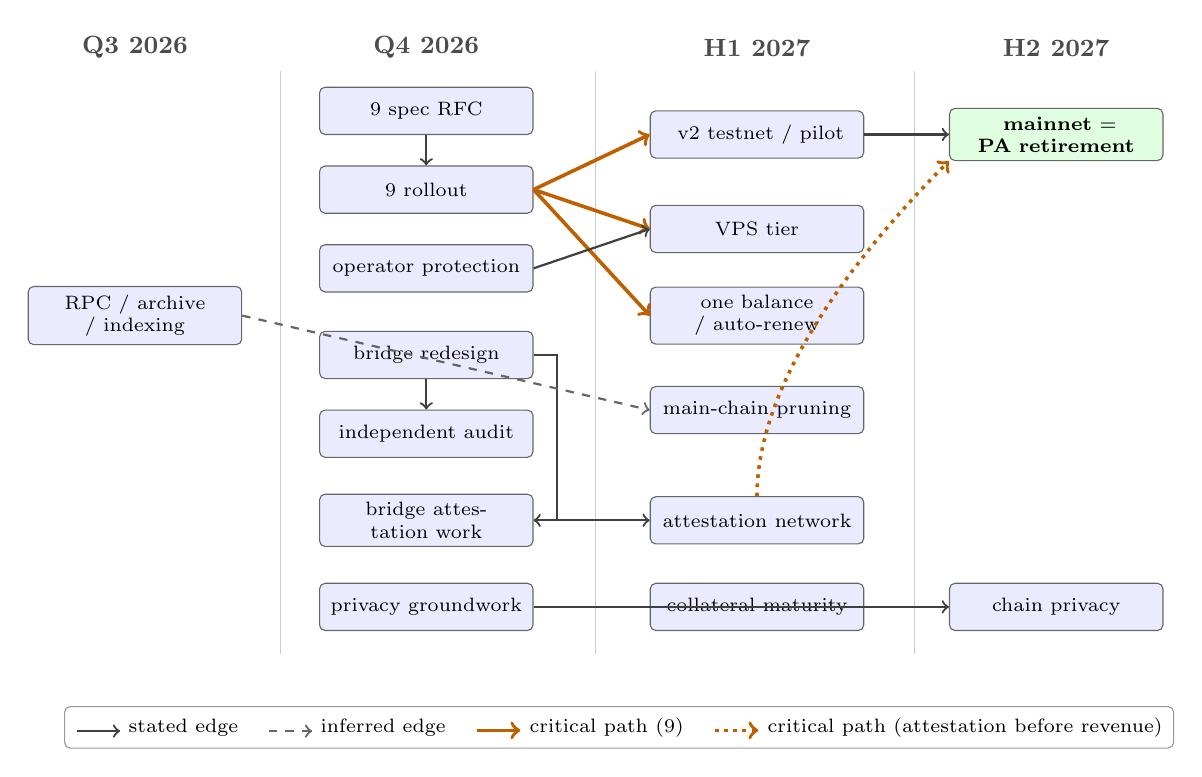
\begin{tikzpicture}[font=\scriptsize,
  n/.style={draw=black!60, rounded corners=2pt, fill=blue!8, align=center, inner sep=3pt,
            text width=2.5cm, minimum height=6mm},
  lane/.style={font=\small\bfseries, text=black!70},
  st/.style={->, thick, black!75},
  inf/.style={->, thick, black!60, dashed},
  cp/.style={->, line width=1.3pt, orange!75!black},
]
\node[lane] at (0,7.0)   {Q3 2026};
\node[lane] at (3.7,7.0) {Q4 2026};
\node[lane] at (7.9,7.0) {H1 2027};
\node[lane] at (11.7,7.0){H2 2027};
\draw[black!20] (1.85,-0.7) -- (1.85,6.7);
\draw[black!20] (5.85,-0.7) -- (5.85,6.7);
\draw[black!20] (9.9,-0.7)  -- (9.9,6.7);

\node[n] (rpc)  at (0,3.6)   {RPC / archive / indexing};
\node[n] (rfc)  at (3.7,6.2) {\specv{9} spec RFC};
\node[n] (v9)   at (3.7,5.2) {\specv{9} rollout};
\node[n] (opro) at (3.7,4.2) {operator protection};
\node[n] (brd)  at (3.7,3.1) {bridge redesign};
\node[n] (aud)  at (3.7,2.1) {independent audit};
\node[n] (att4) at (3.7,1.0) {bridge attestation work};
\node[n] (priv) at (3.7,-0.1){privacy groundwork};

\node[n] (pnr)  at (7.9,5.9) {\PNR{} v2 testnet / pilot};
\node[n] (vps)  at (7.9,4.7) {VPS tier};
\node[n] (bal)  at (7.9,3.6) {one balance / auto-renew};
\node[n] (prun) at (7.9,2.4) {main-chain pruning};
\node[n] (attn) at (7.9,1.0) {attestation network};
\node[n] (coll) at (7.9,-0.1){collateral maturity};

\node[n, fill=green!12] (act) at (11.7,5.9) {\textbf{\PNR{} mainnet $=$ PA retirement}};
\node[n] (chpr) at (11.7,-0.1) {chain privacy};

\draw[st] (rfc) -- (v9);
\draw[cp] (v9.east) -- (pnr.west);
\draw[cp] (v9.east) -- (vps.west);
\draw[cp] (v9.east) -- (bal.west);
\draw[st] (opro.east) -- (vps.west);
\draw[st] (brd) -- (aud);
\draw[st] (brd.east) -- ++(0.3,0) |- (att4.east);
\draw[st] (att4.east) -- (attn.west);
\draw[st] (priv.east) -- (chpr.west);
\draw[st] (pnr.east) -- (act.west);
\draw[inf] (rpc.east) -- (prun.west);
\draw[cp, dotted] (attn.north) .. controls +(0,1.5) and +(-1.1,-1.1) .. (act.south west);

\node[draw=black!40, fill=white, rounded corners=2pt, align=left, inner sep=4pt,
      anchor=south west, font=\scriptsize] at (-0.9,-1.9)
  {\tikz{\draw[st] (0,0)--(0.55,0);} stated edge \quad
   \tikz{\draw[inf] (0,0)--(0.55,0);} inferred edge \quad
   \tikz{\draw[cp] (0,0)--(0.55,0);} critical path (\specv{9}) \quad
   \tikz{\draw[cp,dotted] (0,0)--(0.55,0);} critical path (attestation before revenue)};
\end{tikzpicture}
\caption{Roadmap item dependency graph, clustered by stated quarter.}
\label{fig:e3-depgraph}
\end{figure}

The figure shows the edges of Table~\ref{tab:e3-edges} as a directed graph.


%% =====================================================================
\subsection{Timeline-only items}\label{sec:E4}

\texttt{timeline.html} is a separately hand-authored artifact with its own item set and no prose
counterpart in \texttt{flux-roadmap-public.\allowbreak{}md}; the build pipeline treats the prose document as
the sole source for the rendered PDF and web fragment
\srcdoc{flux-roadmap/public/build-public.sh:7-13}. The 23 items below are reported as a distinct,
lower-weight class of signal — UI tiles, not committed roadmap items — and are never merged into
\S\ref{sec:E1}'s tables.

\begingroup
\footnotesize
\setlength{\tabcolsep}{4pt}
\begin{longtable}{p{0.18\linewidth}p{0.05\linewidth}p{0.13\linewidth}p{0.09\linewidth}p{0.44\linewidth}}
\caption{Items appearing only in \texttt{timeline.html}, reported as weak signals per C12, not commitments.}\label{tab:e4-timeline}\\
\hline
\textbf{Item} & \textbf{Pillar} & \textbf{Maturity} & \textbf{Quarter} & \textbf{Note / citation} \\
\hline
\endfirsthead
\multicolumn{5}{l}{\textit{Table \thetable\ continued}}\\
\hline
\textbf{Item} & \textbf{Pillar} & \textbf{Maturity} & \textbf{Quarter} & \textbf{Note / citation} \\
\hline
\endhead
\hline
\endfoot
\hline
\endlastfoot
bStocks in Zelcore & P8 & IN-PROGRESS & Q3 2026 & \srcroadmap{timeline.html:112-113} \\
Kaspa tokens (``Mass-aware fees $\cdot$ KRC assets'') & P8 & not stated & Q3 2026 & \srcroadmap{timeline.html:115-116} \\
Earn \& staking (``Live APY $\cdot$ Titan'') & P2, P8 & SHIPPED-per-label & Q3 2026 & \srcroadmap{timeline.html:118-119} \\
Fusion transparency (``Per-chain reserves published'') & P8, P2 & not stated & Q3 2026 & \srcroadmap{timeline.html:127-128} \\
SSP Enterprise onboarding (``First marquee clients live'') & P8, P7 & SHIPPED-per-label & Q3 2026 & \srcroadmap{timeline.html:130-131} \\
Flux Foundation (``Ecosystem funding \& governance'') & P7 & not stated & Q3 2026 & \srcroadmap{timeline.html:133-134} \\
FluxAI refocused (``Sellable inference, not chat'') & P6 & not stated & Q3 2026 & \srcroadmap{timeline.html:136-137} \\
Domain Manager overhaul (``Rebuilt $\cdot$ one-click domains'') & P3, P4 & not stated & Q4 2026 & \srcroadmap{timeline.html:175-176} \\
Marketplace push (``Game servers $\cdot$ one-click apps'') & P3 & not stated & Q4 2026 & \srcroadmap{timeline.html:178-179} \\
Inference API (``Paid AI on idle capacity'') & P6 & not stated & Q4 2026 & \srcroadmap{timeline.html:196-197} \\
AI deploy agent (``Chat to deploy $\cdot$ human approval'') & P6 & not stated & Q4 2026 & \srcroadmap{timeline.html:199-200} \\
Zelcore security pack & P8 & not stated & Q4 2026 & Also appears as an H1 2027 sub-item in the prose document. \srcroadmap{timeline.html:202-203} \\
Tax \& CSV export & P8 & not stated & Q4 2026 & Also listed as a sub-item of the Zelcore security pack in \texttt{flux-roadmap-public.\allowbreak{}md}; a separate tile here. \srcroadmap{timeline.html:205-206} \\
SSP Enterprise (``Policy engine $\cdot$ WalletConnect'') & P8, P7 & not stated & Q4 2026 & \srcroadmap{timeline.html:208-209} \\
Transaction screening (``Scam \& drainer warnings'') & P8 & not stated & Q4 2026 & \srcroadmap{timeline.html:211-212} \\
ISO 27001 (``Certification underway'') & P7, P3 & IN-PROGRESS-per-label & Q4 2026 & \srcroadmap{timeline.html:214-215} \\
FluxCore auto-updates (``Self-updating $\cdot$ overclocking controls'') & P1, P9 & not stated & H1 2027 & \srcroadmap{timeline.html:241-242} \\
Torrent application (``Integrated on Flux'') & P3 & not stated & H1 2027 & \srcroadmap{timeline.html:244-245} \\
Fewer, stronger chains (``Long redemption windows'') & P8 & not stated & H1 2027 & Restates the bridge-migration item of Table~\ref{tab:e1-h1} as its own tile. \srcroadmap{timeline.html:247-248} \\
More chains \& assets (``98 chains and growing'') & P8 & SHIPPED-per-label & H1 2027 & The ``98 chains'' figure appears nowhere in \texttt{flux-roadmap-public.\allowbreak{}md}; \notestablished{no corroborating count for parallel-asset chain totals in this paper's corpus}. \srcroadmap{timeline.html:268-269} \\
SSP Key multi-pairing (``One phone, many wallets $\cdot$ CLI'') & P8 & not stated & H1 2027 & Restates the H1 2027 wallets multi-pairing item of Table~\ref{tab:e1-h1} as its own tile. \srcroadmap{timeline.html:274-275} \\
\textbf{New benchmark tool} (``Signed node attestation'') & P1 & not stated & H2 2027 & Bears on \S4 and \S14 together: this paper's benchmark-signature finding is that \texttt{fluxbench}'s result is not bound to the machine that produced it (C13), and this item is the roadmap's own stated fix for exactly that gap (C13). Flagged as the one timeline-only item worth chasing. \srcroadmap{timeline.html:295-296} \\
VPN everywhere (``Windows $\cdot$ Linux'') & P8, P4 & not stated & H2 2027 & Restates the H2 2027 CumulusVPN-platforms item of Table~\ref{tab:e1-h2}, dropping ``Intel macOS.'' \srcroadmap{timeline.html:304-305} \\
\end{longtable}
\endgroup

These items are reported separately, rather than folded into \S\ref{sec:E1}, because the build
pipeline that produces the published PDF and HTML fragment draws only from
\texttt{flux-roadmap-public.\allowbreak{}md}
\srcdoc{flux-roadmap/public/build-public.sh:7-13}: \texttt{timeline.html} is a separately
hand-authored artifact with no equivalent editorial gate, so an item appearing only there carries
materially weaker evidentiary weight than one stated in the prose document.

%% =====================================================================
\subsection{Terminology}\label{sec:E5}

\texttt{notation.tex} is the sole authority for canonical names in this paper; where the roadmap's
own spelling differs from, or is absent relative to, the canonical name, both are given below.

\begingroup
\footnotesize
\begin{longtable}{p{0.22\linewidth}p{0.22\linewidth}p{0.51\linewidth}}
\caption{Roadmap terminology versus this paper's canonical names.}\label{tab:e5-terms}\\
\hline
\textbf{Roadmap's own spelling} & \textbf{Canonical name (\texttt{notation.tex})} & \textbf{Note} \\
\hline
\endfirsthead
\multicolumn{3}{l}{\textit{Table \thetable\ continued}}\\
\hline
\textbf{Roadmap's own spelling} & \textbf{Canonical name (\texttt{notation.tex})} & \textbf{Note} \\
\hline
\endhead
\hline
\endfoot
\hline
\endlastfoot
``FusionX'' (redemption, H1 2027) \srcdoc{flux-roadmap/public/flux-roadmap-public.md:135} and ``Fusion'' (reserve transparency, \texttt{timeline.html}) \srcroadmap{timeline.html:127-128} & \FusionX{} (redemption/exchange product) and \Fusion{} (incumbent custodial bridge) & \texttt{notation.tex} treats these as two distinct canonical names, matching the roadmap's own two distinct usages; the roadmap's bridge-redesign section never names the incumbent bridge it replaces at all, calling it only ``bridge addresses'' \srcdoc{flux-roadmap/public/flux-roadmap-public.md:96-99}. \\
(no tier name used) --- ``operators,'' ``nodes,'' generic ``datacenter tier'' / ``VPS tier'' & \tiers{} = \{\tC{} (\CumulusVPN{} is a product name and is never the Cumulus tier), \tN{}, \tS{}\} & The tier names Cumulus, Nimbus and Stratus appear nowhere in \texttt{public/\allowbreak{}flux-roadmap-public.\allowbreak{}md}, \texttt{public/\allowbreak{}timeline.\allowbreak{}html}, or the PDF text; the canonical names are sourced from \texttt{fluxd}/FluxOS, not from the public roadmap. \\
``FluxCloud'' and ``FluxEdge,'' merged product not separately named \srcdoc{flux-roadmap/public/flux-roadmap-public.md:43} & \FluxCloud{}, \FluxEdge{} & \textbf{Settled: the merged product is \FluxCloud{}} --- ``that's the brand, all available there'' \srcintent{08-answers-round-2.md, round 13}. \FluxEdge{} is retained in this paper only where it names the component as it exists today; the converged product carries the \FluxCloud{} name and no new macro is needed. \\
``PNR v2'' \srcdoc{flux-roadmap/public/flux-roadmap-public.md:111} & \PNR{} (Progressive Node Rewards) & \texttt{notation.tex} flags \PoN{} and \PNR{} as a deliberate terminology hazard: different mechanisms in different layers, trivially confused; both expansions must be given on first use. \\
``FluxOS v9'' / ``v9'' \srcdoc{flux-roadmap/public/flux-roadmap-public.md:52,55} & \specv{9} (the \appspec{} version) & \texttt{notation.tex} reserves ``v9'' exclusively for the application-specification version in this paper; \fluxd{}'s client version 9.1.0 is unrelated and is written out in full, as \daemonversion{}, wherever it appears. \\
``Attestation network'' (opt-in bonded tier, k-of-n verification) \srcdoc{flux-roadmap/public/flux-roadmap-public.md:135} & \SAS{} (System Attestation Service, repo \fluxsas{}) is the \emph{existing} service; the roadmap's bonded network is a distinct, larger, not-yet-built mechanism & The roadmap's item and this paper's \SAS{} share the word ``attestation'' but are not the same mechanism; conflating them is a terminology hazard this paper's evidence flags directly. \\
``VPONs'' / ``Private deployments'' \srcdoc{flux-roadmap/public/flux-roadmap-public.md:83} & \VPON{} (singular macro; private deployment / private overlay network) & The roadmap's plural usage and \texttt{timeline.html}'s ``Private overlay networks'' tile refer to the same singular canonical concept. \\
\end{longtable}
\endgroup

%% Drain this section's float queue before the next begins.
\FloatBarrier
